\documentclass[11pt]{article}
\usepackage{amsmath}
\usepackage{geometry}                % See geometry.pdf to learn the layout options. There are lots.
\geometry{letterpaper}                   % ... or a4paper or a5paper or ... 
%\geometry{landscape}                % Activate for for rotated page geometry
%\usepackage[parfill]{parskip}    % Activate to begin paragraphs with an empty line rather than an indent
\usepackage{graphicx}
\usepackage{amssymb}
\usepackage{epstopdf}
\usepackage{pdflscape}
\DeclareGraphicsRule{.tif}{png}{.png}{`convert #1 `dirname #1`/`basename #1 .tif`.png}
\usepackage{/Library/Frameworks/R.framework/Resources/share/texmf/Sweave}


\title{Foundation species genetics impacts lichen community networks}
\author{M.K. Lau, L.J. Lamit and T.G. Whitham}
%\date{}                                           % Activate to display a given date or no date

\begin{document}
\maketitle

\section{NOTES:}
\begin{enumerate}
\item What network statistics should you use?
\item Run all analyses with only the N45-55.
\item Enter data from Pit
\item 
\item If sending to PLoS, use the AZ Science Foundation gradate assistance grant.
\end{enumerate}

\section{Summary}

\begin{itemize}
\item Interactions among species are important determinants of biodiversity through both ecological and evolutionary processes.
\item Bark lichen communities offer a unique study system for exploring the genetic underpinnings of inter-specific interactions due to the spatial and temporal scales at which they operate.
\item Here we examine the potential for interactions among lichen species to be influenced by the genetics of a foundation species (\textit{Populus aungustifolia}). 
\item Three main findings emerged:
	\begin{enumerate}
	\item Co-occurrence analysis indicate that species relationships were primarily aggregative, indicative of facilitative relationships
	\item Community network structure differed between sampling heights (45-55cm and 80-90cm) with the higher sampling height having fewer connections among species
	\item Community network structure varied significantly among genotypes; however this depended on the location that the communities were sampled on the tree
	\end{enumerate}
\item These results suggest that community assembly and/or interactions among lichen species can be influenced by the genetics of a foundation species; however these effects are dependent upon variation within individuals.
\end{itemize}



\section{Methods and Results}

\subsection{Sampling}
\begin{itemize}
\item Data were collected from a common garden of replicated \textit{P. angustifolia} clones at the Ogden Nature Center (Ogden, UT) in May 2010 and 2011.
\item The presence of lichen species was assessed within 50 1cm$^2$ cells in a 10cm$^2$ grid arrayed in a checkerboard pattern, chosen in accordance with the average thallus size of the largest lichen 
(data?) to avoid overlapping lichen thalli between cells.
\item The $\gamma$ diversity of the study was 9 species. These lichen species were crustose and foliose with the dominant lichen species being the foliose (\textit{Xanthomendoza galericulata}.
\item Quadrats were surveyed on the north side of each replicate tree at two heights: 45-55cm and 80-90cm.
\item Modeling and analyses were conducted in R. 
\end{itemize}

\subsection{Co-Occurrence Analysis}

\begin{itemize}
\item Co-occurrence analysis was conducted to test for significant patterns of either segregative (e.g., competitive) or aggregative (e.g., facilitative) relationships among species.
\item Each quadrat on a tree (45-55cm and 80-90cm) was analyzed separately for co-occurrence patterns.
\item Stone and Roberts (1990) c-score was used because of its performance in null-model based co-occurrence analysis and interpretability of community-wide patterns of co-occurrence.
\item To test for significance we used a sequential swap randomization algorithm that maintained species totals but allowed observation totals to vary.
\item A total of 10,000 randomizations with a 500 iteration burn-in were used to calculate a standardized effect size (i.e., (c-score$_{observed} - \mu_{simulated}) \ \div \ sd_{simulated}$) and a P-value for each quadrat.
\item SES did not vary significantly among genotypes, but there was an overall trend of negative SES values indicating aggregation (i.e., species tended to occur together more often than expected under the null-model) (Fig. 1).
\end{itemize}

\subsection{Community Network Modeling}

\begin{itemize}
\item Community networks were modeled for each quadrat by testing for significant, non-linear correlations among species using Kendall's Tau.
\item Network structure, measured by the number of connections in the network (size) and the distribution of connections among species (centralization; 0 = all species have equal numbers of connections to 1 = one species is connected to all other species), was analyzed by testing for the effect of genotype and quadrat position (i.e., 45-55cm and 80-90cm) nested within tree individuals (see Table 1).
\item The lower (45-55cm) quadrat had more connections on average than the upper quadrat (80-90cm) (Fig. 2).
\item Both the size and centralization of the community networks varied significantly among among genotype; however this depended on the position of the quadrat on the tree (Fig 3; also see code for analyses).
\end{itemize}

\newpage

\begin{figure}[h]
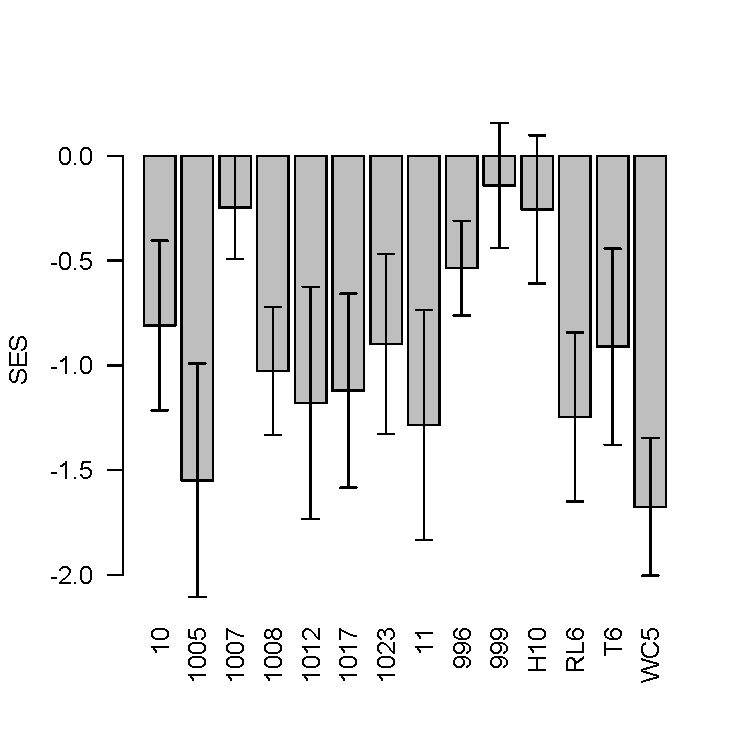
\includegraphics[width=9.5cm,height=9.5cm]{fig1.pdf}
\caption{The mean standardized effect size (SES) $\pm$ 1 S.E. for each genotype.}
\end{figure}

\newpage

\begin{figure}[h]
\begin{center}
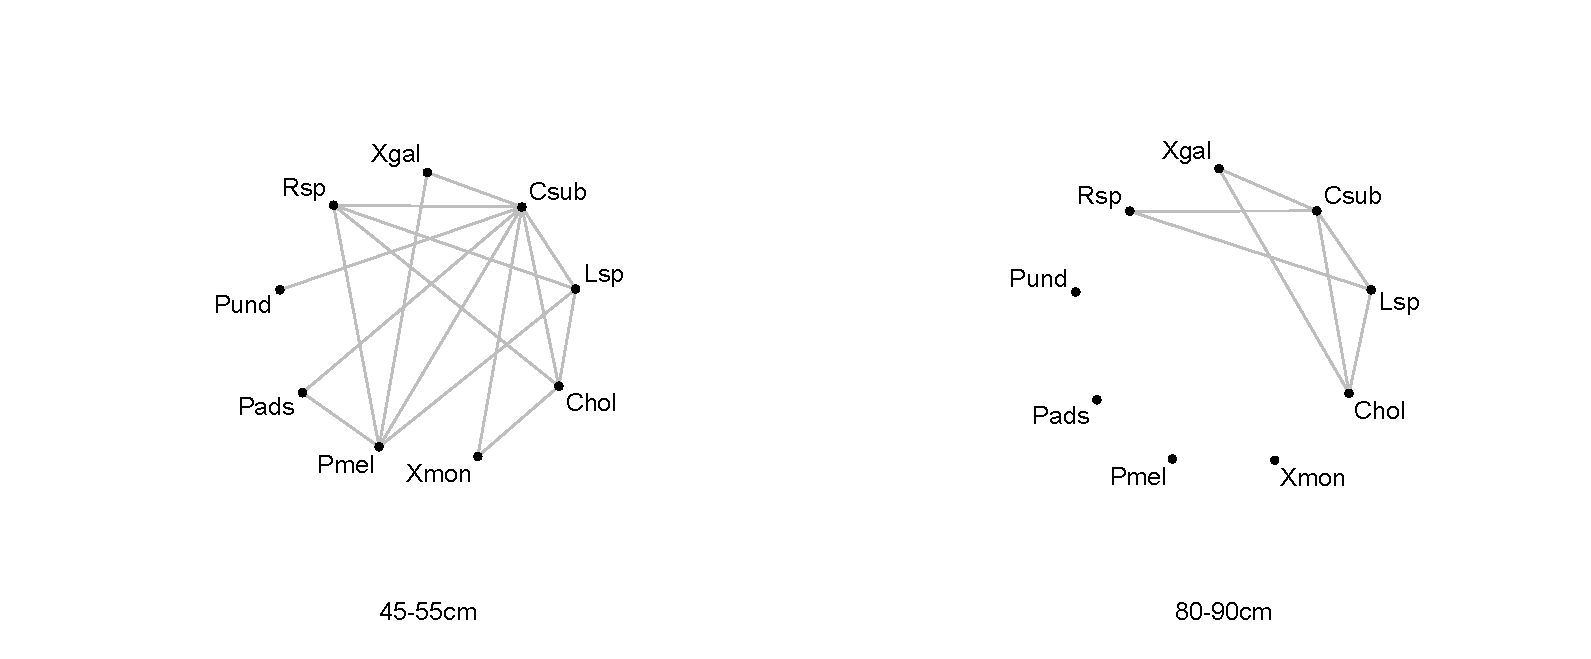
\includegraphics[width=16.5cm,height=7.5cm]{fig2.pdf}
\caption{Network graphs for the lower (45-55cm) and upper (80-90cm) quadrats. Connections in the graphs are the average across all network models for quadrats at their respective heights.}
\end{center}
\end{figure}

\newpage

\begin{figure}[h]
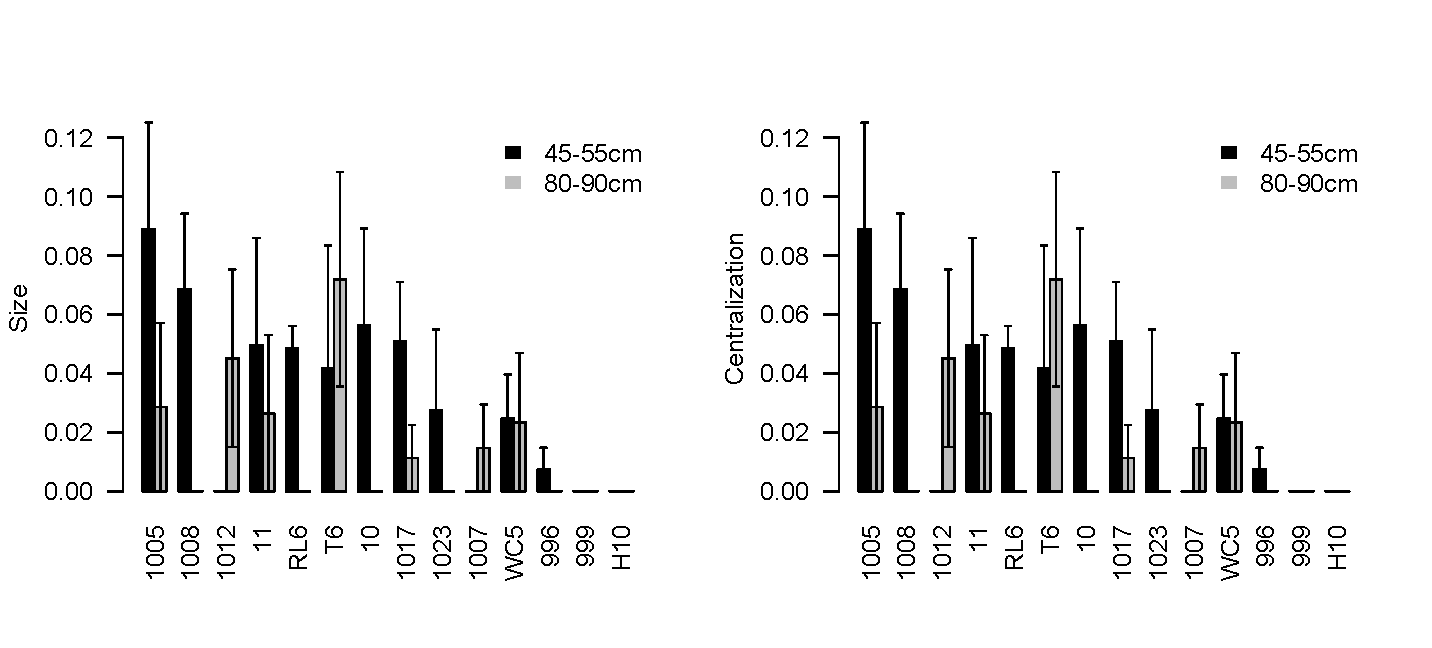
\includegraphics[width=16.5cm,height=7.5cm]{fig3.pdf}
\caption{The mean size and centralization scores  $\pm$ 1 S.E. for each genotype by quadrat position.}
\end{figure}

\newpage

\begin{table}[h]
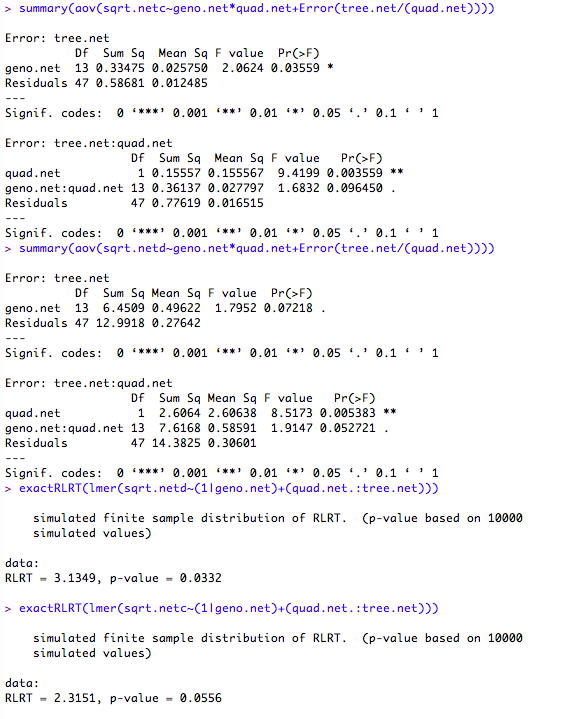
\includegraphics[scale=1]{Routput}
\caption{Analysis and output for the network statistics. Variable object names: \texttt{sqrt.netc} = square root transformed network centralization, \texttt{sqrt.netc} = square root transformed network size, \texttt{geno.net} = genotype of each network model, \texttt{quad.net} = quadrat location, \texttt{tree.net} = tree identifier. Note that the REML model is not outputting the effects of each factor. I'm actually not sure how to do this.}
\end{table}

\newpage
\section*{Screen Only Analyses}

\begin{figure}[h]
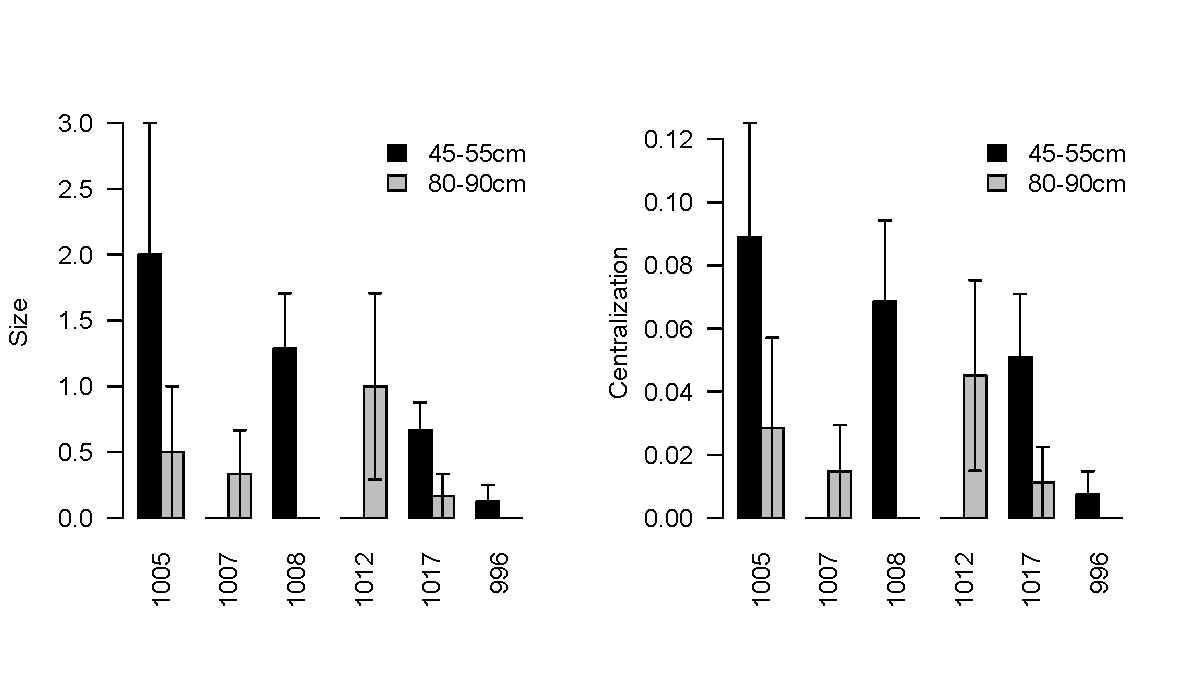
\includegraphics[width=16.5cm,height=7.5cm]{screenFig.pdf}
\caption{The mean size and centralization scores  $\pm$ 1 S.E. for each genotype by quadrat position for the genotypes from the Screen site only.}
\end{figure}

\begin{table}[h]
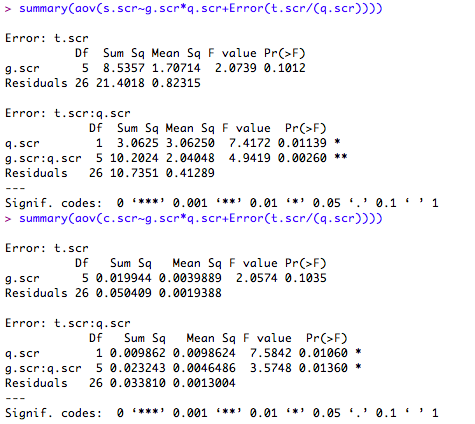
\includegraphics[scale=1]{screen}
\caption{Analysis and output for the network statistics for the genotypes from the Screen site only.}
\end{table}

\newpage

\begin{figure}[h]
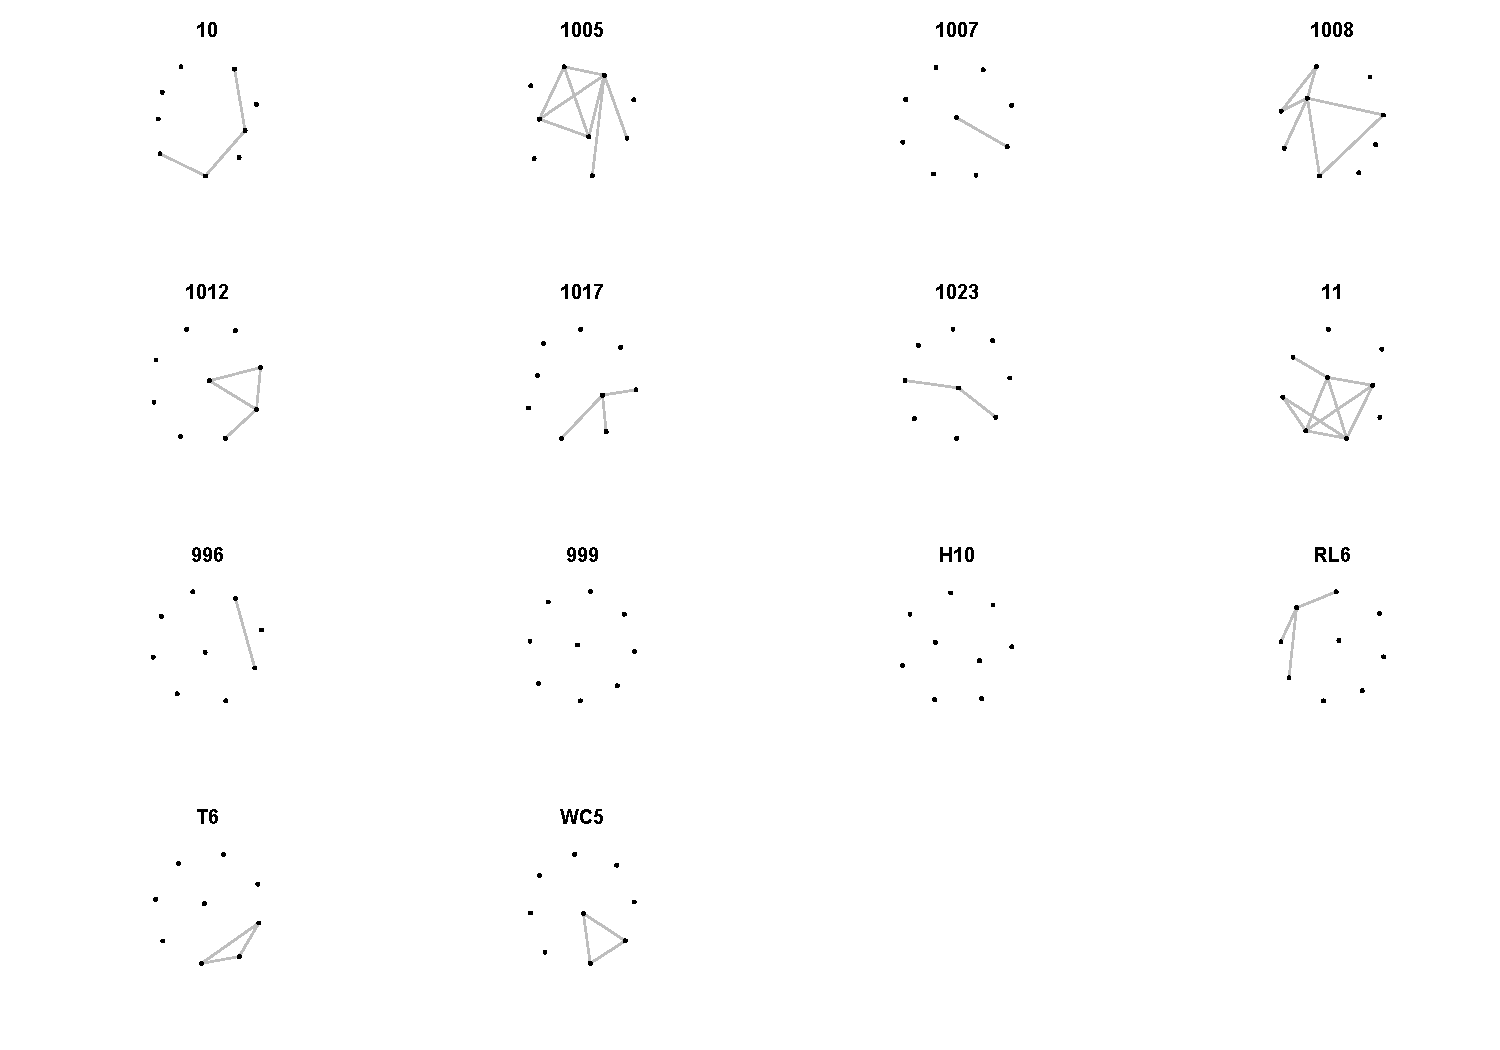
\includegraphics[width=18cm,height=12.5cm]{genonets}
\caption{Network graphs for each genotype where the connections are averages of replicate networks for each genotype.}
\end{figure}


\end{document}  